%% LyX 2.3.3 created this file.  For more info, see http://www.lyx.org/.
%% Do not edit unless you really know what you are doing.
\documentclass[language=finnish,version=final,mainfont=none,sharelatex=false,hidechapters=true,countbibpages=false,emptyfirstpages=true,minted=true]{utuftthesis}
\setcounter{secnumdepth}{2}
\setcounter{tocdepth}{2}
\usepackage{float}

\makeatletter

%%%%%%%%%%%%%%%%%%%%%%%%%%%%%% LyX specific LaTeX commands.
\providecommand\textquotedblplain{%
  \bgroup\addfontfeatures{Mapping=}\char34\egroup}
%% Because html converters don't know tabularnewline
\providecommand{\tabularnewline}{\\}
\floatstyle{ruled}
\newfloat{algorithm}{tbp}{loa}
\providecommand{\algorithmname}{Algoritmi}
\floatname{algorithm}{\protect\algorithmname}

\@ifundefined{showcaptionsetup}{}{%
 \PassOptionsToPackage{caption=false}{subfig}}
\usepackage{subfig}
\makeatother

\renewcommand{\listingscaption}{Ohjelmalistaus}

\addbibresource{Bibliografia.bib}
\begin{document}
\begin{comment}
Document template suitable for use as a LaTeX master-file for master's
thesis in University of Turku Department of Future Technologies.\\
\\
Compatible with: ShareLaTeX, pdfLaTeX, LuaLaTeX, XeLaTeX, LyX, latexmk.
The document class is described in utuftthesis.cls.\\
\\
HOW TO USE? See https://gitlab.utu.fi/ttweb/thesis
\end{comment}

\pubyear{2020}

\pubmonth{11}

\publab{Tietojenkäsittelytiede}

\publaben{Computer Science}

\pubtype{luk}
\title{Linux-palvelinten tietoturva}
\author{Maks Turtiainen}

\maketitle
\keywords{Tietoturva, Linux, Palvelin}
\begin{abstract}
    Miten Linux-palvelinylläpitäjä voi suojautua tietoturvauhilta? Tutkielman haasteena on tarkastella keinoja suojautua tyypillisimmiltä kyberhyökkäyksiltä Linux-palvelinympäristössä. Palvelimiin kohdistunut kyberhyökkäys voi johtaa erittäin tuhoisiin seurauksiin ja Linux-käyttöjärjestelmä on yleisin alusta palvelimissa. Näistä syistä tutkielma tarkastelee keinoja suojautua kyberhyökkäyksiltä nimenomaan Linux-palvelimien näkökulmasta.
\end{abstract}


% empty pagestyle for table of contents etc.
% otherwise you'll get simple page style with roman page numbers
\pagestyle{empty}

% mandatory
\tableofcontents

% if you want a list of figures
\listoffigures

% if you want a list of tables
% \listoftables

% if you want a list of acronyms
\listofacronyms


% change the name if the default doesn't sound right
\renewcommand{\algorithmname}{Ohjelmalistaus}% 'list of X'
%   - it is also possible to define custom lists
%     \chapter{List Of Xs} 
%   - the secnumdepth trickery is needed because acronyms are as a
%     standard chapter and we are faking '\listofacronyms'
%
%\setcounter{secnumdepth}{-1}
%\input{your acronym chapter's file name}
%\setcounter{secnumdepth}{2}% setup page numbering, page counter, etc.%
\begin{comment}
The thesis starts here.

To better organize things, create a new tex file for each chapter
and input it below.

Avoid using the å, ä, ö or <space> characters in referred names and
underscores \_ in file names (may break hyperref).

Good luck!
\end{comment}

\makeatletter
\newcommand{\customlabel}[2]{%
   \protected@write \@auxout {}{\string \newlabel {#1}{{#2}{\thepage}{#2}{#1}{}} }%
   \hypertarget{#1}{}
}
\makeatother
\chapter{Johdanto}\label{Johdanto}

    Palvelimen vaarantunut tietoturva voi asettaa alttiiksi tuhansien, jopa miljoonien ihmisten tietoja. Liiketoiminnan kontekstissa palvelimen tietoturvan pettäminen voi johtaa miljoonien eurojen menetykseen liiketoimintakriittisen sovelluksen ollessa pois käytöstä. Pahimmillaan voidaan puhua ihmishenkien menetyksen vaarasta kun kyseessä on esimerkiksi terveydenhuollon infrastruktuuriin kuuluva palvelin. Palvelinten tietoturvaa voi edellä mainittujen seikkojen vuoksi pitää huomattavasti tärkeämpänä kuin esimerkiksi tavallisen työpöytätietokoneen.

    Palvelinten tietoturva on tärkeää myös palvelinten luonteen vuoksi. Palvelimen on oltava helposti saatavilla asiakassovelluksilleen. Palvelimen suora saatavuus internetissä ja palvelut, joita palvelin ajaa, luovat palvelimen hyökkäyspinta-alasta korkeamman kuin esimerkiksi tavallisen työpöytätietokoneen.

    Valtaosa palvelimista käyttää käyttöjärjestelmänään Linuxia. W3Cookin analyysin mukaan jopa 96,4 \% julkisista web-palvelimista käyttää Linux-käyttöjärjestelmää\cite{w3cook}. Tästä syystä tutkielma keskittyy nimenomaan Linux-palvelinten tietoturvaan.

    Tutkielmani haasteena on esitellä kuinka Linux-palvelimen ylläpitäjä voi suojautua tyypillisimmiltä tietoturvauhilta. Toisessa luvussa johdattelen Linuxin ja palvelinten perusteisiin, jonka jälkeen luvussa 3 käyn läpi tärkeimpiä konsepteja tietoturvasta puhuttaessa ja tyypillisimpiä tietoturvauhkia sekä kyberhyökkäyksiä. Luvussa 4 esittelen kuinka näiltä tietoturvauhilta ja kyberhyökkäyksiltä voi suojautua.

\chapter{Linux ja palvelimet}\label{linux_ja_palvelimet}

\section{Linux}\label{linux}

Linux on perhe käyttöjärjestelmiä, jotka perustuvat Linux käyttöjärjestelmäytimeen eli kerneliin. Linux-kernelin ensimmäisen version julkaisi Linus Torvalds vuonna 1991 opiskellessaan Helsingin Yliopiston Tietojenkäsittelytieteen laitoksella. Linux-käyttöjärjestelmällä viitataan mihin tahansa Linux-kerneliä käyttävään käyttöjärjestelmään. Linux on UNIX-tyyppinen käyttöjärjestelmä, mutta ei jaa samaa koodikantaa UNIX-käyttöjärjestelmien kanssa, ei ole sertifioitu eikä noudata Single UNIX Specification -standardia. Linux-kerneliä käyttävät käyttöjärjestelmät paketoidaan yleensä Linux-jakeluksi, jotka useimmiten sisältävät kernelin lisäksi kokoilman ohjelmistoja sekä paketinhallinnan. Linux-kerneli ja useimmat Linux-jakelut ovat vapaata lähdekoodia.~\cite{openbookos}~\cite{mediumlinux}

Työpöytäkäytössä Microsoft Windows on suosituin käyttöjärjestelmä, Linuxia käyttävät vuonna 2020 vain 1,74\% työpöytäkäyttäjistä.~\cite{statcounter}~ Mobiililaitteissa suosituin käyttöjärjestelmä on Googlen Android, jonka voi katsoa olevan Linux-jakelu sen käyttäessä muokattua versiota Linux-kernelistä.~\cite{itworld} Mobiililaitteista Androidia käytti 85 \% vuonna 2018~\cite{cnet}. Vuosina 2017–2019 maailman 500 tehokkaimmasta supertietokoneesta kaikki käyttävät Linuxia.~\cite{itsfoss}. Internetin julkisista web-palvelimista vuonna 2015 Linuxia käyttää 69,7\%-96,4\% riippuen lähteestä.~\cite{w3techs}~\cite{w3cook}

Linux-jakeluiden kotisivujen käyttäjämäärien perusteella suosituimmat 3 Linux-jakelua ovat MX Linux, Manjaro ja Mint (21.10.2020).~\cite{distrowatch} Useimpien Linux-jakeluiden vapaan saatavuuden vuoksi on vaikea arvioida todellisia käyttäjämääriä, mutta suosituimpia Linux-jakeluita palvelinkäytössä lienevät Red Hat Enterprise Linux, SuSE, Ubuntu, Debian sekä CentOS.~\cite{linuxcom}

Perusteita suurelle Linuxin käytölle palvelimissa on arvioitu olevan vakaus ja luotettavuus, turvallisuus, muokattavuus, lähdekoodin avoimuus sekä kustannukset.~\cite{tecmint}

\section{Palvelimet}\label{palvelimet}

Palvelin on tietokonejärjestelmä, joka tarjoilee palveluja, dataa tai muita resursseja asiakastietokoneilleen– tai sovelluksilleen, useimmiten internetin välityksellä. Palvelimet koostuvat yleensä palvelinkäyttöön tarkoitetusta tietokoneesta sekä palvelinkäyttöön tarkoitetusta käyttöjärjestelmästä. Erityyppisiä palvelimia ovat mm.\ tiedostopalvelimet, tulostinpalvelimet, sovelluspalvelimet, DNS-palvelimet, sähköpostipalvelimet, tietokantapalvelimet ja web-palvelimet.

Järjestelmän arkkitehtuuria, jossa palvelin palvelee asiakaskonetta, kutsutaan asiakas–palvelin malliksi. Tyypillisesti palvelimet ja asiakkaat keskustelevat keskenään pyyntö– ja vastausperiaatteella. Asiakas lähettää pyynnön palvelimelle, johon palvelin vastaa. Esimerkiksi asiakkaan web-selain lähettää HTTP-pyynnön palvelimelle, johon palvelin vastaa HTML:n muodossa.

Käytännössä mikä tahansa tietokone voi olla palvelin, mutta yleensä palvelimet ovat palvelinkäyttöön tarkoitettuja tietokoneita, jotka sijaitsevat palvelinsalissa. Palvelintietokoneet koostuvat osista, jotka ovat luotettavampia kuin kuluttajatietokoneissa. Useimmiten palvelintietokoneet ovat räkkiin sopivassa vaakamallisessa kotelossa ja räkissä palvelimia voi olla useita kymmeniä. Suurimmissa palvelinsaleissa voi olla satoja räkkejä. Palvelin ei tarvitse näyttöä tai syöttölaitteita kuten näppäimistöä tai hiirtä muuta kuin huoltotoimenpiteissä, joten tilan ja kustannusten säästämiseksi näitä harvemmin on palvelimissa. Palvelinta kontrolloidaan etänä esimerkiksi SSH:n välityksellä, web-pohjaisesta käyttöliittymästä tai jollakin kaupallisella ratkaisulla kuten Microsoft Managment Consolella.~\cite{paessler}

Palvelintietokoneissa osien kokoonpano pyrkii mahdollisemman suureen toimintavarmuuteen. Tekniikoita joilla toimintavarmuutta pyritään takaamaan ovat muun muassa virheenkorjaava muisti (ECC), osien lennosta vaihto, kriittisten osien tuplana saatavilla oleminen, RAID–levyjärjestelmät sekä virransyötön takaaminen akustolla (UPS) tai jopa generaattoreilla. Tyypillinen palvelin pysyy toimintakykyisenä vaikka siitä hajoaisi virtalähde tai tallennuslaite kuten kovalevy tai vaikka koko rakennuksesta katkeaisivat sähköt.

Palvelin voi olla myös toisen palvelimen tarjoama virtuaalipalvelin. Tässä tapauksessa fyysinen palvelin toimii virtuaalipalvelinalustana ja voi ylläpitää useita kymmeniä virtualisoituja käyttöjärjestelmiä. Nykyisin virtuaalipalvelinalusta koostuu useista fyysisistä palvelimista tai jopa palvelinsaleista ja resursseja pystyy allokoimaan virtuaalipalvelimille joustavasti (klusterointi).

Käytännössä varsinaisten fyysisten palvelinten ja palvelinsalien ylläpito on keskittynyt muutamille suurille palveluntarjoajille, joilla on käytössään useita kymmeniä palvelinsaleja. Harvat palvelinresursseja tarvitsevat ylläpitävät itse omia fyysisiä palvelimiaan omissa tiloissaan. Tyypillisesti resurssit vuokrataan palveluntarjoajalta. Palvelinresurssit voivat olla virtuaalipalvelimia, fyysisiä palvelimia palveluntarjoajan tiloissa tai pääsy yhteisessä käytössä olevalle palvelimelle.~\cite{virtualizationfordummies}

\section{Tyypillinen Linux-palvelinkonfiguraatio}\label{tyypillinen_palvelinkonfiguraatio}

    Esittelen seuraavaksi kuvitteellisen, mutta realistisen esimerkin palvelinarkkitehtuurin toteutuksesta laitteistosta ohjelmistoihin, loppukäyttäjästä ylläpitoon. Päämääränä on tarjota palvelinresurssit keskisuuren yrityksen web-sovellukselle.

    Yritys vuokraa palveluntarjoajalta virtuaalipalvelimen. Palveluntarjoajalla on useita suuria palvelinsaleja. Kyseisen virtuaalipalvelimet tarjoillaan yhdestä palvelinsalista jossa on 100 kpl räkkejä, joissa jokaisessa on 10 palvelintietokonetta. Yksittäisen räkin varavirtalähteenä on akusto, joka sijaitsee räkin alaosassa. Koko palvelinsalin varavirranlähteenä toimii diesel-aggregaatti. Palvelinsalin palvelintietokoneista on allokoitu virtuaalipalvelinten vuokraamiseen 10 räkin eli 100 palvelintietokoneen verran. Palvelintietokoneet ovat identtisiä keskenään. Suuren kapasiteetin tarpeen vuoksi niissä on useampi prosessori sekä runsaasti virheenkorjaavaa keskusmuistia. Tallennustilana toimii 10 SSD-levyä. Levyt ovat kytketty RAID 6 järjestelmään tarjoten näin tallennustilaa 80\% levykapasiteetista kahden levyn redundanssilla. Levyt on lennosta vaihdettavia, joten levyn rikkoontuessa palvelimen toiminta ei keskeydy. Yhdessä palvelinkoneessa on 2 lennosta vaihdettavaa virtalähdettä.

    Virtuaalipalvelinalustat käyttävät Red Hat Enterprise Linuxia käyttöjärjestelmänään. Virtualisointiin käytetään vapaan lähdekoodin QEMU–projektia. Virtuaalikoneita on keskimäärin 10 yhdellä fyysisellä palvelimella.

    Asiakasyritys vuokraa yhden virtuaalipalvelimen, jolle allokoidaan 1/10 fyysisen palvelimen resursseista. Virtuaalipalvelimen käyttöjärjestelmänä on Ubuntu Linux. Virtuaalipalvelinta ohjataan SSH-yhteiden välityksellä. Yriyksen web-sovellus on Python–ohjelmointikielellä kirjoitettu. Web-applikaatiokirjastona on käytetty Djangoa. Djangon sisäinen HTTP-palvelinsovellus tarjoilee sisällön ainoastaan IP:lle 127.0.0.1 porttiin 3000. Samalla virtuaalipalvelimella ajetaan myös Nginx–nimistä HTTP-palvelinta, joka toimii käänteisenä välityspalvelimena paikallisen HTTP-palvelimen ja ulkoverkon välillä. Nginx HTTP-palvelin välittää Django-palvelimen 3000 portin ulkoverkkoon porttiin 80 ja 443.

    Palvelinresursseja vuokraava yritys tarjoaa myös DNS-nimipalveluita. Virtuaalipalvelimen IP:lle allokoidaan esimerkki.fi domain.

    Asiakasyrityksen web-sovellus on nyt saatavilla HTTP (S) -protokollan ylitse esimerkki.fi osoitteesta portista 80 tai 443. Asiakasyrityksen asiakkaat vierailevat web-selaimellaan osoitteessa esimerkki.fi. Asiakkaan tietokone lähettää ensin DNS-tiedustelun ja saa vastaukseksi virtuaalipalvelimen IP-osoitteen. Tämän jälkeen web-selain lähettää HTTP–pyynnön kyseiseen IP:seen porttiin 80. Virtuaalipalvelimella pyörivä Nginx välittää pyynnön Djangon HTTP-palvelimelle, joka vastaa pyyntöön HTML-koodilla. Nginx välittää tämän HTML:n takaisin asiakkaan web-selaimelle ja web-selain renderöi HTML-koodista web-sivuston.

\chapter{Tietoturva}\label{tietoturva}

Tietoturvalla tarkoitetaan tietokonejärjestelmien ja verkkojen suojelemista elektronisten resurssien varkauksilta, ohjelmistojen ja laitteiden vahingoilta sekä tahallen aiheutetuilta häiriöiltä palvelujen toimintakyvyssä. Suojautumaan pyritään myös palvelujen väärinkäytöksiltä. Tietoturvan merkitys on kasvanut nopeasti digitalisaation myötä.~\cite{definitionofcyber}

\section{CIA-malli}\label{cia_malli}

Tärkeimpiä konsepteja tietoturvasta puhuttaessa on luottamuksellisuus, eheys sekä saatavuus. Tämän johdosta yksi tärkeimmistä malleista kuvata tietoturvan osa-alueita on CIA-malli (Confidentality, Integrity, Availability). Malli antaa viitekehyksen keskustellessa siitä, millainen jokin tietoturvauhka on. Mallin mukaisesti jokin tietoturvauhka kohdistuu aina yhteen tai useampaan CIA-mallin osa-alueista.~\cite{basicsofinformationsecurity}

\begin{figure}
\centering 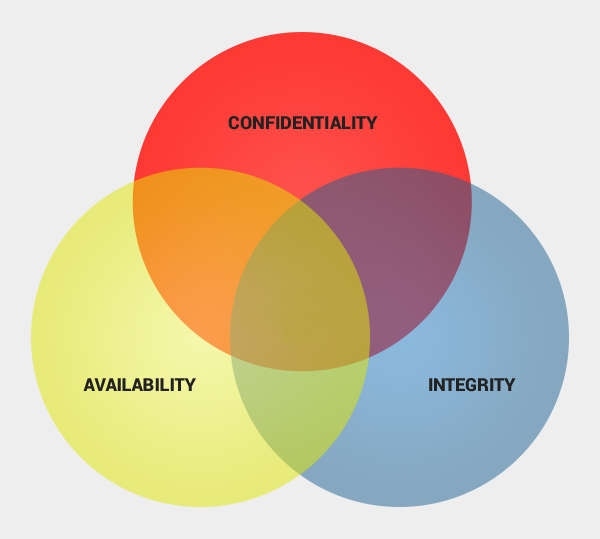
\includegraphics[width=0.5\textwidth]{kuvat/cia.png}
\caption{CIA-malli}
\label{cia} 
\end{figure}

\section{Haavoittuvuudet ja kyberhyökkäykset}\label{haavoittuvuudet_ja_kyberhyokkaykset}
Tietoturva-aukolla eli haavoittuvuudella tarkoitetaan heikkoutta tietokonejärjestelmässä, jonka avulla hyökkääjän on mahdollista päästä tekemään järjestelmässä jotakin mitä hänen ei pitäisi. Kyberhyökkäys tarkoittaa varsinaista toimenpidettä jossa hyökkääjä käyttää haavoittuvuutta päästäkseen järjestelmään.~\cite{nist}

Esittelen seuraavaksi yleisimpiä kyberhyökkäyksiä, mitä haavoittuvuutta ne hyödyntävät ja mitä CIA-mallin kohtaa ne vaarantavat. Merkitsen jokaisen esittelemäni hyökkäyksen tunnisteella ja numeroinnilla Hx, jotta niihin on helpompi palata myöhemmissä luvuissa.

\subsection{H1: Palvelunestohyökkäys}\customlabel{dos}{H1}
Palvelunestohyökkäyksen (eng. Denial of Service, DoS) tarkoitus on saada jokin verkossa oleva resurssi pois käytöstä häiritsemällä tätä internetin välityksellä. Tyypillisesti tämä saavutetaan häiritsemällä kohdetta lukuisilla palvelupyynnöillä joiden tarkoitus on saada resurssi ylikuormitettua, jonka jälkeen tavalliset resurssin käyttäjät eivät enää pääse tähän käsiksi. Palvelunestohyökkäys estää palvelun saatavuuden, joten se hyökkää CIA-mallin A-kohtaan.~\cite{nist_ddos}

Palvelintietokoneella on lukuisia rajallisia resursseja kuten kaista, levytila tai suoritinaika. Hyökkääjä voi esimerkiksi lähettää toistuvasti palvelupyyntöjä ladatakseen suuren tiedoston palvelimelta ja näin ollen tukkia kaistan tai hyökkääjä voi lähettää toistuvia palvelupyyntöjä johonkin resurssiin, jonka tietää olevan raskas suorittemelle ja näin ollen ylikuormittaa suorittimen.

Todellisuudessa harvalla hyökkääjällä on käytössään sellaisia resursseja, joilla olisi mahdollista tukkia jonkin kaupallisen toimijan palvelinresurssit. Tämän vuoksi nykyään yleisempi tapa on toteuttaa palvelunestohyökkäys on tehdä se hajautetusti (DDoS, Distibuted Denial of Service). Hajautetussa palvelunestohyökkäyksessä hyökkääjällä on käytössään useista internetiin yhdistetyistä tietokoneista muodostuva bottiverkko. Näiden tietokoneiden hallinnan hyökkääjä on saanut aikaisemmin jollakin muulla kyberhyökkäyksellä. Bottiverkossa voi olla mukana jopa satoja tuhansia tietokoneita ja tällaisen verkon haltija voi lähettää toistuvia pyyntöjä kaikilta verkon tietokoneilta samaan aikaan. Näin massiivisen verkon haltija voisi ylikuormittittaa esimerkiksi tyypillisen verkkosivuston vain yksinkertaisesti lataamalla jokaisella verkon koneella toistuvasti verkkosivustoa.~\cite{informationsecurity}

Tällaisiä ``raakaan voimaan'' perustuvia palvelunestohyökkäyksiä vastaan voi olla vaikea suojautua. Useimmat nykyaikaiset reitittimet osaavat jo jättää hyökkääjän liikenteen huomiotta, mikäli toistuvat palvelupyynnöt tulevat samasta lähteestä. Tilanne onkin toinen kun pyynnöt tulevat useista tuhansista lähteistä samaan aikaan. Tyypillisesti isoilla palveluntuottajilla on vain yksinkertaisesti niin paljon resursseja, että näitä on hyvin vaikea kenenkään tukkia. Toinen vaihtoehto on tehdä suunnitelma sen varalta, jos palvelunestohyökkäys tapahtuu. Tällaiseen suunnitelmaan voi kuulua replikaa palvelusta joka otetaan käyttöön hyökkäyksen sattuessa.

``Raa'an voiman'' käyttö palvelunestohyökkäyksissä on yksinkertaisin ja yleisin tapa, mutta palvelunestohyökkäys voidaan toteuttaa myös muilla keinoilla. Muita keinoja ovat osoitintietojen muuttaminen ja virheellisten palvelupyyntöjen lähetys sen toivossa, että palvelu kaatuu.

Kuvassa \ref{github_ddos} toistaiseksi toiseksi suurimman palvelunestohyökkäyksen piikki kaistankäytössä hyökkäyksen aikana. Hyökkäys on vuodelta 2018 ja se kohdistui Githubiin. Poikkeuksellisesti hyökkäyksessä ei käytetty bottiverkkoa vaan hyökkääjä vahvisti omia häirintäpyyntöjään tuhansilla väärinkonfiguroiduilla Memcached-palvelimilla.~\cite{wired_github_ddos}

\begin{figure}
\centering 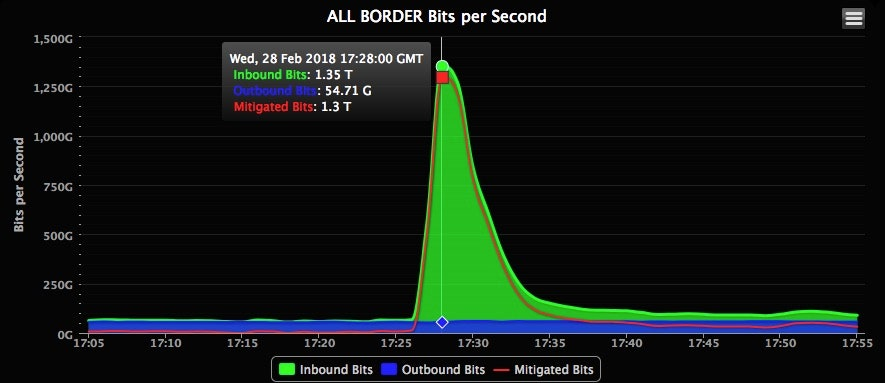
\includegraphics[width=1\textwidth]{kuvat/github_ddos.jpg}
\caption{Github DDoS 2018}
\label{github_ddos} 
\end{figure}

\subsection{H2: Takaovet}\customlabel{backdoors}{H2}
Takaovi (eng. Backdoor) on keino ohittaa järjestelmän tyypilliset autentikointimenetelmät. Tyypillisesti takaovi on tietokoneohjelma joka antaa hyökkääjälle hallinnan kohdejärjestelmästään. Esimerkiksi Linux-järjestelmässä takaovella yritetään saada tilanne aikaan jossa hyökkääjä voi kirjautua sisään kohdejärjestelmälle root-oikeuksilla käymättä kuitenkaan normaalia autentikaatioprosessia läpi. Tässä tapauksessa hyökkääjällä on täysi kontrolli kohdejärjestelmästä, joten hyökkäys voi kohdistua kaikkiin CIA-mallin osa-alueisiin.~\cite{wired_backdoor}

Takaovi asennetaan kohdetietokoneelle esimerkiksi nk.\ troijalaisen mukana. Troijalainen on viattomaksi naamioitu haittaohjelma, esimerkiksi peli, jonka mukana on kuitenkin ohjelmakoodia joka ei kuulu peliin kuten esimerkiksi takaovi.

Takaovia asennetaan myös jo muilla keinoin onnistuneen hyökkäyksen päätteeksi taatakseen hyökkääjällä pääsyn kohdejärjestelmään tulevaisuudessa.

\subsection{H3: Verkon kuuntelu}\customlabel{verkon_kuuntelu}{H3}
Verkon kuuntelu on keino salakuunnella jotakin tahoa analysoimalla verkkoliikennettä. Useimmiten liikenne on salattu joten ensin on onnistuttava murtautumaan salauksen läpi. Liikenne voi myös kulkea kaapeleita pitkin joihin pääsy on fyysisesti estetty ja itse verkkoliikenne on salaamatonta. Verkon kuuntelulla lähtökohtaisesti hyökätään CIA-mallin C-kohtaan, sillä hyökkääjä näkee tietoja jotka eivät ole hänen katseltavakseen tarkoitettu. Verkon kuuntelun tuloksena voidaan saada käsiin tietoja, joilla onnistutaan tekemään jokin muu kyberhyökkäys.

Langattomien verkkojen aikana verkon kuuntelu ei vaadi enää fyysistä pääsyä kaapeleihin, joten tarpeeksi suurella vastaanottimella hyökkääjä voi toteuttaa hyökkäyksen mistä vain. Tätä ongelmaa on korjattu vahvoilla salauksilla langattomassa verkkoliikenteessä. Varsinkin WLAN:n alkuaikoina salaukset olivat heikkoja tai niitä ei ollut lainkaan ja tämä oli suuri ongelma.

\subsection{H4: Näppäilytallennin}\customlabel{keylogger}{H4}
Näppäilytallennin (eng. Keylogger) on laite tai tietokoneohjelma joka tallentaa kaikki kohteen näppäinpainallukset ja joko lähettää ne reaaliajassa hyökkääjälle tai hyökkääjä voi hakea esimerkiksi piilotetun laitteen kohteesta. Näppäinpainallusten tallennuksella tarkoituksena on useimmiten hankkia salaiseksi tarkoitettuja tietoja, kuten salasanoja. Näppälytallennin kohdistuu CIA-mallin C-kohtaan, sillä hyökkääjä yrittää saada tietoja, joita hänen nähtäväkseen ei oltu tarkoitettu.

\subsection{H5: Koodin etäsuoritus}\customlabel{remote_code_execution}{H5}
Koodin etäsuoritus (eng. Remote Code Execution)

\subsection{H6: Eskalaatiohyökkäys}\customlabel{privilege_escalation}{H6}
Eskalaatiohyökkäys (eng. Privilege escalation)

\subsection{H7: Väsytyshyökkäys}\customlabel{bruteforce}{H7}
Väsytyshyökkäys (eng. Brute-force)

\subsection{H8: Laitteen varkaus}\customlabel{theft}{H8}
Laitteen varkaus

\chapter{Kyberhyökkäyksiltä suojautuminen}\label{suojautuminen}

Vaikka keskityn tutkielmassani ensisijaisesti Linux–palvelinten tietoturvan parantamiseen, monet yleiset keinot tietoturvan parantamiseen pätevät myös Linux–palvelinten kontekstissa joten käsittelen myös niitä lopuksi lyhyesti.

\section{Salaus}\label{Salaus}
Tallennustila ja tietoliikenne voidaan kryptografisesti salata. Salaamalla sekokielistä tietoa muutetaan muotoon, jossa vain tarvittavan avaimen haltija pystyy lukemaan tietoja selkokielisinä.

Salaamalla tietoa voidaan estää päätymästä sellaisiin käsiin mihin se ei ole tarkoitettu. Salauksella vahvennetaan tietoturvaa CIA-mallin C-kohdan osalta. Salaamisella voidaan suojautua tietojen päätymiseltä vääriin käsiin esimerkiksi tietokoneen varkauden tai verkon kuuntelun yhteydessä.

\subsection{Tallennustilan salaaminen}\label{tallennustilan_salaaminen}
Tallennustilan tai yksittäisten tiedostojen salaamisella pyritään ehkäisemään tietojen päätyminen vääriin käsiin tilanteessa jossa laite, jolle tieto on tallennettu, päätyy tahoille joiden ei ole tarkoitus nähdä tietoja. Tilanne on tämä esimerkiksi hyökkäyksessä \ref{theft}. Tallennustilan tai tiedostojen salaamisella voidaan myös pyrkiä suojelemaan jotakin erittäin salaista osaa tiedoista jonka salausta pidetään purettuva vain silloin kun tietoja tarvitaan. Tälläisessä tapauksessa tietojen on mahdollista pysyä pois vääristä käsistä jopa silloin kun hyökkääjä on saanut muutoin täyden hallinnan tietoja säilyttävästä palvelimesta, kuten hyökkäyksissä \ref{backdoors}, \ref{remote_code_execution} ja \ref{bruteforce}.

DMCrypt on Linux-kernelin levysalausjärjestelmä. Järjestelmä on osa laajempaa Device Mapper rajapintaa josta järjestelmän nimikin on johdettu (\textbf{D}evice \textbf{M}apper \textbf{crypt}). Device Mapper on rajapinta jolla voi osoittaa virtuaalisia laitetiedostoja fyysisiin laitetiedostoihin. Tätä teknologiaa DMCrypt hyödyntää salauksessaan. Varsinainen levyosion tai laitteet laitetiedosto on salattu ja sellaisenaan käyttökelvoton. Purkaessaan salauksen DMCrypt luo virtuaalisen laitetiedoston jossa tieto on selkokielisenä ja tämä virtuaalinen osio on valmis liitettäväksi järjestelmään.

Cryptsetup on työkalu levysalauksien hallintaan DMCryptillä. Useita standardeja siitä, missä muodossa salatut osiot tulee olla on useita ja Cryptsetup tukee näistä LUKS:ia, loop-AES:ia, TrueCryptiä ja Microsoftin BitLockeria. Salatun osion muoto määrittelee esimerkiksi sen millainen osion alun salaamaton ylätunniste on. Ylätunniste kertoo lyhyesti ohjeet salauksen purkamiseen, esimerkiksi sen, mitä salausalgoritmia salaukseen on käytetty. Cryptsetup tukee myös ylätunnisteettomia nk. paljaita DMCrypt-osioita. LUKS:ia tyypillisesti suositellaan Linux-järjestelmän osioita salatessa.

Ohjelmalistauksessa~\ref{alg:cryptsetup_salaus} esimerkki levyosion salaamisesta Cryptsetupilla käyttäen salausavaimena salasanaa. Salattava osio on lohkolaitetiedosto \textit{/dev/sda2} ja se on tarkoitus liittää hakemistopuun sijaintiin \textit{/home}.

\begin{algorithm}[tbh]
\begin{minted}{sh}
# Ensin alustetaan osio LUKS-muotoon (syötä haluttu salasana)
cryptsetup luksFormat /dev/sda2
# Puretaan juuri salatun osion salaus ja anna sille virtuaalinen nimi
cryptsetup open /dev/sda esim
# Nyt virtuaalinen laitetiedosto on saatavilla polussa /dev/mapper/esim
# Alustetaan tiedostojärjestelmä virtuaaliselle laitetiedostolle
mkfs.ext4 /dev/mapper/esim
# Nyt virtuaalisella laitetiedostolla on tiedostojärjestelmä
# ja sen voi liittää normaalisti hakemistopuuhun
mount /dev/mapper/esim /home
\end{minted}
\caption{Levyosion salaus Cryptsetupilla.\label{alg:cryptsetup_salaus}}
\end{algorithm}
\newpage{}

Tietoa voi salata myös tiedostotasolla. Tiedostotason salaukseen on useita työkaluja kuten eCryptFS ja EncFS. eCryptFS on toteutettu Linuxin kerneliin kuten DMCrypt. EncFS on käyttäjätilassa toimiva erillinen sovellus ja huomattavasti helppokäyttöisempi. EncFS:n käyttö on varsin suoraviivaista, ohjelmalistauksessa \ref{alg:encfs_salaus} salataan hakemisto \textit{/home/user/salattava} ja säilötään salattu data hakemistoon \textit{/home/user/.salattu}.

\begin{algorithm}[tbh]
\begin{minted}{sh}
# Salatun hakemiston luonti ja olemassa olevan salatun
# hakemiston salauksen purku tapahtuu samalla komennolla
encfs /home/user/.salattu /home/user/salattava
\end{minted}
\caption{Levyosion salaus EncFS:llä.\label{alg:encfs_salaus}}
\end{algorithm}
\newpage{}

\subsection{Tietoliikenteen salaaminen}\label{tietoliikenteen_salaaminen}

Tietoliikenteen salaamisella pyritään ensisijaisesti suojautumaan hyökkäykseltä \ref{verkon_kuuntelu}. Useimmiten tietoliikenteen salaaminen on jonkin tiedonvälitykseen käytettävän protokollan tehtävä (esim. HTTP vs. HTTPS) ja merkityksellisintä turvallisen tiedonvälityksen kannalta on tehdä turvallisia sovellusvalintoja. Esimerkiksi on suositeltavaa tehdä Linux-palvelimen ylläpitotoimia etäyhteydellä ennemmin salatun SSH:n kuin salaamattoman Telnetin välityksellä.

On myös mahdollista toteuttaa kokonaisvaltaisempaa tietoliikenteen salaamista tunneloimalla tietoliikenne jonkin salatun teknologian lävitse. Tällöin voidaan varmistua, että liikenne on salattua, vaikka käyttäjätasolla käytettäisiinkin protokollaa, joka ei tue salausta. Yleisin tähän tarkoitukseen käytetty teknologia on salattu VPN. Implementaatioita VPN:stä on lukuisia ja toiminta niiden välillä eroaa paljonkin. Linux-palvelinylläpidon näkökulmasta käytännöllisin implementaatio lienee OpenVPN.

OpenVPN:n avulla voidaan TCP/UDP tasolla tunneloida kaikki tietoliikenne salatun IP-tunnelin ylitse.

\section{Palomuurit}\label{palomuurit}
Palomuuri on järjestelmä, jonka tarkoitus on estää asiaton pääsy verkkojen välillä. Useimmiten tämä toteutetaan

\section{SELinux}\label{selinux}
SELinux (Security Enhanced Linux) on Red Hat Enterprise Linuxin\ldots

\section{Kernelitason suojaus}\label{kernelitason_suojaus}
Linuxin kerneli tarjoaa monia työkaluja suojella\ldots 

\section{Eristys ja virtualisointi}\label{eristys_ja_virtualisointi}
Vaikka Linux-kerneli tarjoaa keinoja eristää sovelluksia, on usein tarpeen toteuttaa eristys virtualisoinnin avulla.

\subsection{Virtualisoinnin työkaluja}\label{virtualisoinnin_tyokaluja}
Virtualisointi jaetaan useimmiten kahteen pääkategoriaan; kokonaiseen virtualisointiin jossa koko tietokoneen laitteisto simuloidaan sekä ns. paravirtualisointiin jossa ohjelmistot ajetaan omassa eristetyssä ympäristössä simuloimatta kuitenkaan tietokoneen komponentteja.
Alustoja laitteiston virtualisointiin Linuxilla ovat mm. KVM (Kernel-based Virtual Machine), VMWare, VirtualBox, XEN, QEMU sekä helpottamaan virtualisoinnin ylläpitoa libvirtd.
Paravirtualisointiin alustaja ovat mm. Docker, Vagrant ja Linuxin chroot-ympäristö.

\section{Järjestelmän ja sovellusten konfiguraatio}\label{sovellusten_konfiguraatio}

\subsection{Autentikaatio}\label{autentikaatio}

\chapter{Yhteenveto}\label{yhteenveto}

Tarkastelun kohteena oli muutamia yleisimpiä kyberhyökkäyksiä ja keinoja vahventaa Linuxin tietoturvaa. Esitellyt keinot vahventaa Linux-palvelinten tietoturvaa tarjoavat vähintään vähäistä suojaa esitellyiltä kyberhyökkäyksiltä.

Taulukkoon~\ref{tab:security-table} on koottu käsitellyt hyökkäykset suhteessa suojautumismenetelmiin. Iso \textbf{X} tarkoittaa sitä, että suojautumismenetelmä auttaa merkittävästi suojautumaan tietoturvahyökkäykseltä. Pieni \textbf{x} tarkoittaa puolestaan sitä, että menetelmä auttaa suojautumaan hieman tietoturvahyökkäykseltä. Pienen \textbf{x}:n merkintää käytetään myös silloin, jos suojautumismenetelmä auttaa merkittävästi vähentämään tietoturvahyökkäyksen aiheuttamaa vahinkoa.

Kuten taulukosta~\ref{tab:security-table} huomaa, esitellyt suojautumismenetelmät tuntuvat jakautuvan kahden pääryhmän välillä. Ensimmäisen ryhmän suojautumismenetelmät auttavat tehokkaasti, mutta vain yhteen tiettyyn kyberhyökkäykseen. Kun taas toisen ryhmän menetelmät ovat kokonaisvaltaisempia ratkaisuja, jotka auttavat monilla osa-alueilla hieman.

Taulukosta~\ref{tab:security-table} huomataan myös, että joltakin hyökkäyksiltä on hankala suojautua. Tällainen hyökkäys on esimerkiksi palvelunestohyökkäys~(\ref{dos}). Hyökkäykseltä~\ref{dos} pystytään palomuurien (luku \ref{palomuurit}) avulla suojautumaan vain mikäli hyökkäys tulee yhdestä lähteestä, ennalta arvattavista lähteistä tai muutoin ennalta-arvattavalla tavalla.

\begin{table}
\centering{}\caption{Hyökkäykset vs. suojautumismenetelmät\label{tab:security-table}}
\begin{tabular}{c|c|c|c|c|c|c|c|}
   &\ref{dos}&\ref{backdoors}&\ref{verkon_kuuntelu}&\ref{privilege_escalation}&\ref{injection}&\ref{bruteforce}&\ref{theft} \tabularnewline\hline
    Tallennustilan salaaminen~(\ref{tallennustilan_salaaminen}) & & & & & & & \textbf{X}\tabularnewline\hline
    Tietoliikenteen salaaminen~(\ref{tietoliikenteen_salaaminen}) & & & \textbf{X} & & & &\tabularnewline\hline
    Palomuurit~(\ref{palomuurit}) & \textbf{x} & & & & \textbf{x} & \textbf{x} &\tabularnewline\hline
    Eristys ja virtualisointi~(\ref{eristys_ja_virtualisointi}) & & \textbf{x} & & \textbf{x} & \textbf{x} & \textbf{x} &\tabularnewline\hline
    Autentikaatioprosessin vahvennus~(\ref{autentikaatio}) & & & & & & \textbf{X} &\tabularnewline\hline
    Käyttöoikeuksien vahvennus~(\ref{access_rights}) & & \textbf{x} & & \textbf{x} & \textbf{x} & &\tabularnewline\hline
\end{tabular}
\end{table}


\printbibliography

\end{document}
